\documentclass[a4paper, 12pt]{examen}

\begin{document}

%\modulo{Prog. multim. y de dispositivos moviles}
%\modulo{Planif. y adm. de redes}
%\modulo{Prog. de servicios y procesos}
\modulo{Lenguajes de marcas}

%%%%%%%%%%%%%%%%%%%%%%%%%%%%%%%%%%%%%%%%%%%%%%%%%%%%%%%%%%%%
%%%%%%%%%%%% Recuerda guardar el fichero como ISO-8859-1
%%%%%%%%%%%%%%%%%%%%%%%%%%%%%%%%%%%%%%%%%%%%%%%%%%%%%%%%%%%%

\pregunta{Dado el HTML que puedes encontrar al final y que no se puede modificar, maquetarlo usando rejillas de la manera que indica la figura 1. Aparte de eso hacer lo siguiente:
\begin{itemize}
\item{Cambiar el tipo de letra de todos los h1 para que adopten el tipo Courier.}
\item{Cambiar el color utilizado por el texto en las cajas 1 y 4. Hacer adem�s que el texto est� justificado por ambos m�rgenes.}
\item{Modificar el espacio entre el texto y el borde de las cajas que lo contienen y ajustarlo a 20px.}
\end{itemize}
}{2.5}
\begin{figure}[h]
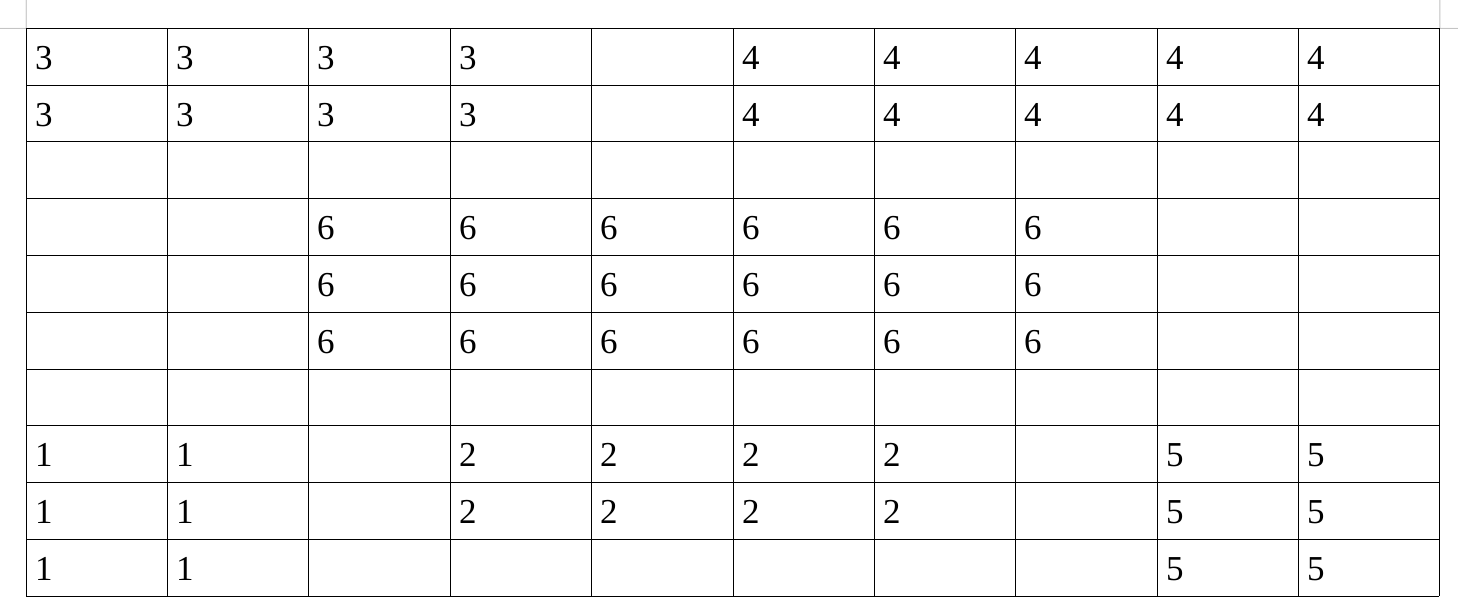
\includegraphics[scale=0.3]{Rejilla.png}
\end{figure}
\pregunta{Dado el mismo HTML que aparece al final construir una maquetaci�n que se adapte a las distintas resoluciones de la manera siguiente:
\begin{itemize}
\item{El fondo de la p�gina siempre es un archivo de imagen llamado ``fondo.jpg''}
\item{En pantallas grandes (de 801px o m�s) se desea que usando float los elementos aparezca como indica la figura 2}
\item{En pantallas peque�as (de 800px o menos) se deber�n mostrar los elementos simplemente apilando unos encima de otros, en el mismo orden (1,2,3,4,5 y 6) y con un tipo de letra m�s grande}
\end{itemize}
En este ejercicio est� permitido a�adir cajas pero no modificar el orden de las ya existentes.
}{5.5}

\begin{figure}[h]
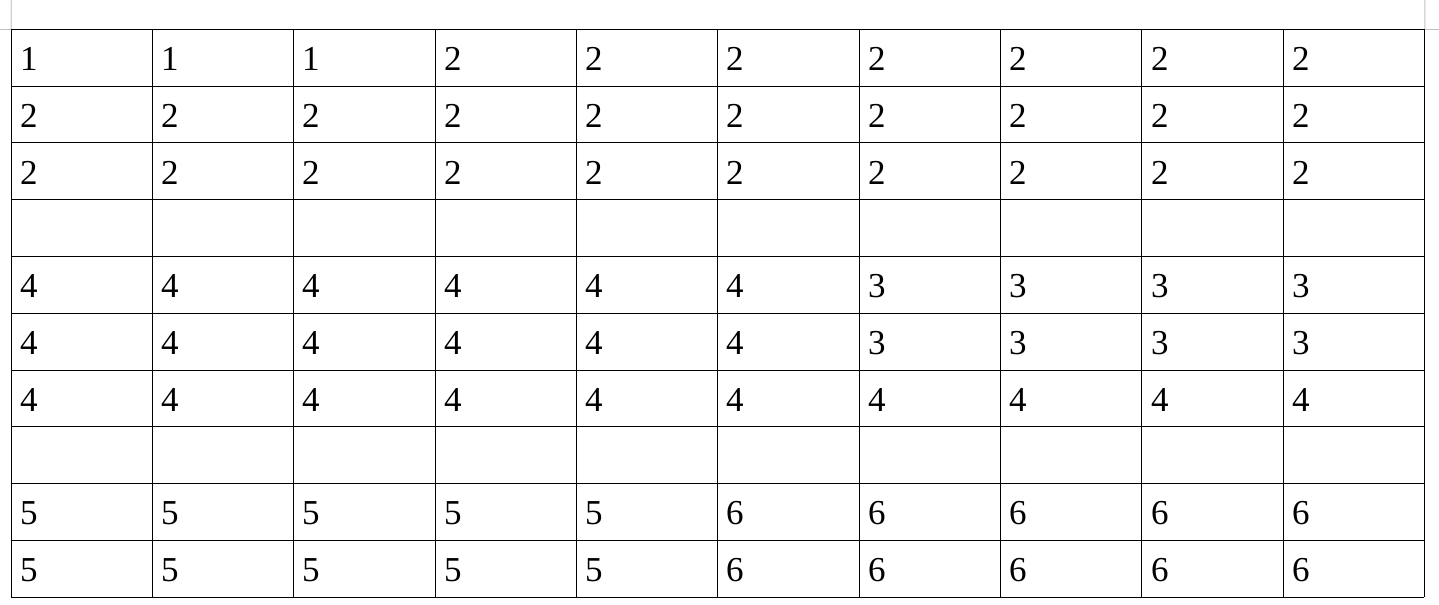
\includegraphics[scale=0.3]{Float01.png}
\end{figure}


\break

\begin{verbatim}
<div id="contenedor">
    <div id="caja1">
        <h1> Caja 1 </h1>
        Texto ...
    </div>
    <div id="caja2">
        <h1> Caja 2</h1>
        Texto ...
    </div>
    <div id="caja3">
        <h1>Caja 3</h1>
        Texto ...
    </div>
    <div id="caja4">
        <h1>Caja 4</h1>
        Texto ...
    </div>
    <div id="caja5">
        <h1>Caja 5</h1>
        Texto ...
    </div>
    <div id="caja6">
        <h1>Caja 6</h1>
        Texto ...
    </div>
</div>

\end{verbatim}

\pregunta{Dada la tabla HTML que se muestra (y que no se puede modificar) usar CSS para conseguir que se muestre como indica la figura:}{2}
\begin{itemize}
\item{El fondo de las cabeceras es azul y el color de las letras es blanco.}
\item{Consigue los bordes que se muestran en la figura.}
\item{La tabla se ha decorado variando las filas pares e impares.}
\item{Si se pasa el rat�n por las celdas de una fila, todas las celdas de dicha fila cambian de color para ayudar al usuario a ver en qu� fila est� situado.}
\end{itemize}
\begin{figure}[h]
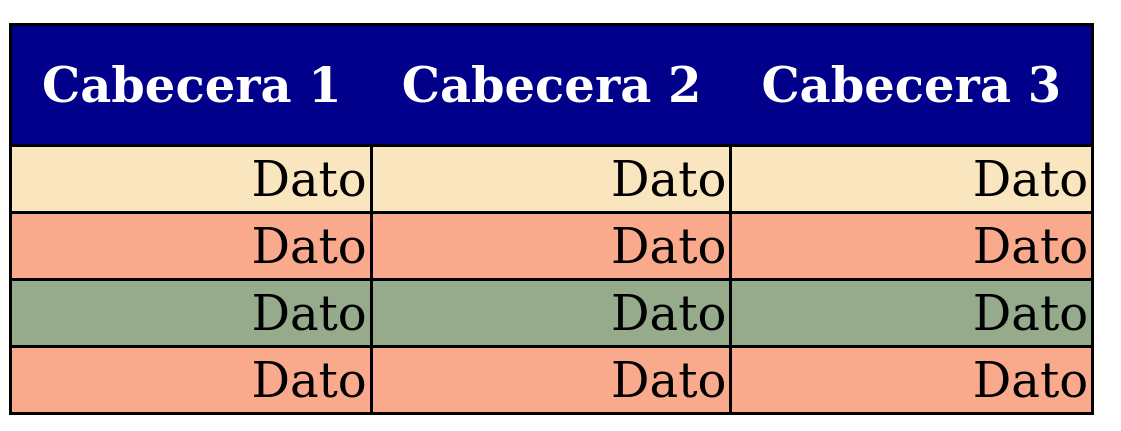
\includegraphics[scale=0.3]{Tabla01.png}
\end{figure}

\end{document}
